\subsection{Configuration Module}
\label{sec:ConfigurationModule}

Configuration Module functions the configuration of fuzzy concepts over crisp database, negation and quantification of natural language. The crisp database is the one load it in the Loading File Module. Users are entitled to create and edit fuzzy concepts such as ``beautiful", ``old" by defining fuzzy functions over attributes in crisp database. Negations and quantifications can be created by defining the their functions over unit interval $[0,1]$.

\subsubsection{Fuzzy Concept}
Fuzzy concept is created over one of attributes in crisp database. For example, we can create fuzzy concept ``expensive" over attribute ``price". In this section, we formalize definition of fuzzy concept.
\begin{defin} \textbf{Fuzzy Concept}
Let $\mathcal{A}$ be a set of attributes, and $\mathcal{D}$ be a set of domain, that is $\mathcal{D}=\{(type, range) \mid type =\{Continuous, Discrete\}\}$. $g_{AD}$ is a function mapping  from attributes to domains, that is, $\mathcal{A} \rightarrow \mathcal{D}$. Suppose there existes fuzzy function $f_{D}$ is $\mathcal{D} \rightarrow [0,1]$. 

A fuzzy concept $FC$ is defined as a function $f_{FC}: \mathcal{A} \rightarrow [0,1]$. Indeed, $f_{FC}(att)= f_{D}(g_{AD}({att}))$, where $att \in \mathcal{A}$.
\end{defin}
\begin{ex} \textbf{Create fuzzy concept ``big"}
\label{ex:CreateFuzzyConcept}
As shown in house.xml, there exists an attribute ``size"  with its type ``Continuous (C)" and its range ``[(0,2500]]", which means an interval from 0 to 2500.
\begin{lstlisting}
<AttrDom>
	<Attribute>size </Attribute> 
	<Domain>
		<Type>C</Type>
		<Range>[(0,2500]]</Range> 
	</Domain>
</AttrDom>
\end{lstlisting}

A fuzzy concept ``big" can be created over attribute ``size" by defining fuzzy functions from domain [(0,2500]] to [0,1]. For example, 

\[
  big(x) = \left\{ 
  \begin{array}{l l}
  	0.002000 \times x & \quad x \in (0.000000,50.000000] \\
    	0.003333 \times x-0.066667& \quad x \in (50.000000,80.000000]  \\
    	0.002500 \times x & \quad x \in (80.000000,120.000000] \\
   	0.001250 \times x+0.150000 & \quad x \in (120.000000,200.000000] \\
    	0.001000 \times x+0.200000 & \quad x \in (200.000000,500.000000]  \\
    	0.000200 \times x+0.600000 & \quad x \in (500.000000,1500.000000]  \\
	0.000100 \times x+0.750000 & \quad x \in (1500.000000,2500.000000]  \\
  \end{array} \right.
\]
\end{ex}

\subsubsection{Fuzzy Quantification}
Fuzzy quantifier can be defined as second order fuzzy relations, which is formalized as $D: \mathcal{F}(U)^n \longrightarrow [0,1]$, where $U$ is domain of interest, and $\mathcal{F}(U)$ is a set of all fuzzy subsets of $U$. In natural language, most of the statements with quantifiers takes less than $3$ or $4$ fuzzy subsets as arguments,  such as ``very tall pretty girls", ``extremely strict professors". We express the simplest statements taking $2$ fuzzy subsets as parameters, then quantifier $Q$ is defined as a function $Q: \mathcal{F}(U) \times \mathcal{F}(U) \longrightarrow [0,1]$. In most of such statements, the last concept is not really fuzzy one, but crisp. Normally, the value of quantifier function will not be affected by the crisp concept. The statement ``All men are tall." is expressed as \[\textbf{all}(\textbf{men},\textbf{tall}) = inf\{max(1-\textbf{men}(e), \textbf{tall}(e)), e \in U \}\],  where the value of \textbf{men} doesn't actually affect on the final result. There is a linguistics reason here. In computational linguistics, dependency among words are considered as foundation to apply linguistics function over those words. For example, in statement ``very tall men", ``very" and ``men" are not dependent on each other, but ``very" and ``tall" have dependency, so do ``tall" and ``persons". Therefore, the quantifier function ``very" is not defined dependent on crisp set ``men" according to the linguistics meaning. 

Thus, we redefine quantifier without considering the crisp concept. It is formalized as $Q: \mathcal{F}(U) \longrightarrow [0,1]$. Even though, this definition is still a second order fuzzy set. In order to implement quantification in RFuzzy Framework, we need first order fuzzy predicate.

\begin{defin} \textbf{Fuzzy Quantification defined in First Order Fuzzy Predicate}
Let $U$ be a set of fuzzy concepts, which is simply a set of names of fuzzy concepts. $f : U \rightarrow [0,1]$ is function of fuzzy concept. $\mathcal{F}(U)$ is the set of all functions of all fuzzy concepts. $Q$ is a set of quantifications, which was defined as $Q: \mathcal{F}(U) \longrightarrow [0,1]$.
At present, for an arbitrary quantification $q \in Q$, for each fuzzy concept $c \in U$, we create a new quantificion $q_{c}: [0,1] \rightarrow [0,1]$, where the first $[0,1]$ is the range of function $f_{c}$ of fuzzy concept $c$ .
\end{defin}

\begin{ex} \textbf{Create quantification ``very" for fuzzy concept ``big"}
As shown in the example \ref{ex:CreateFuzzyConcept}, ``big" is a fuzzy concept and its function is $f(big)$. Suppose \textit{very} is a fuzzy quantifier. Then we create a new fuzzy quantifier $very_{big}$, which is a function $[0,1] \rightarrow [0,1]$.
\[  very_{big}(x) = \left\{ 
  \begin{array}{l l}
    0 & \quad \text{if 0 $0 \leq x < 0.4$}\\
    7/8*x & \quad \text{if $0.4 \leq x < 0.8$}\\
    x & \quad \text{if $0.8 \leq x \leq 1.0$}\\
  \end{array} \right.
\]
\end{ex}

\subsubsection{How to use interface of Configuration Module}
There are several configurations for users, which are shown in table \ref{tab:configurations}. 

\begin{table}[b]
\begin{center}
\begin{tabular}{|c|c|c|c|}
\hline
     & Add & Remove & Edit \\  
\hline
Fuzzy Concept & \ding{52}&  \ding{52}&  \ding{52}\\
\hline
Fuzzy Negation& \ding{52}&  \ding{52}&  \ding{52}\\
\hline
Fuzzy Quantification & \ding{52}&  \ding{52}&  \ding{52}\\
\hline
Concept Functions& \ding{52}&  \ding{52}&  \ding{52}\\
\hline
Negation Functions& \ding{52}&  \ding{52}&  \ding{52}\\
\hline
Quantification Functions& \ding{52}&  \ding{52}&  \ding{52}\\
\hline
\end{tabular}
\end{center}
\label{tab:configurations}
\caption{Operations in Configuration Module}
\end{table}

\newpage
\begin{figure}[h]
\begin{center}
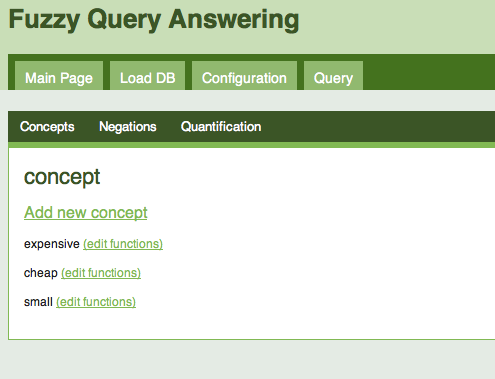
\includegraphics[scale=0.6]{Configuration.png}
\end{center}
\caption{Interface of Configuration Module}
\label{fig:CMI}
\end{figure}
As shown in figure \ref{fig:CMI}, the existing fuzzy concepts, negations and quantifications are shown by clicking subtitles ``Concepts", ``Negations" and ``Quantifications", respectively. In each page, users can click ``Add New concept", ``Add New negation" and ``Add New Quantification" to enter Adding pages.  Users can click hyperlink ``edit function" behind the fuzzy concept, negation or quantification you want to edit to enter the Editing page.
\newpage
\begin{figure}[h]
\begin{center}
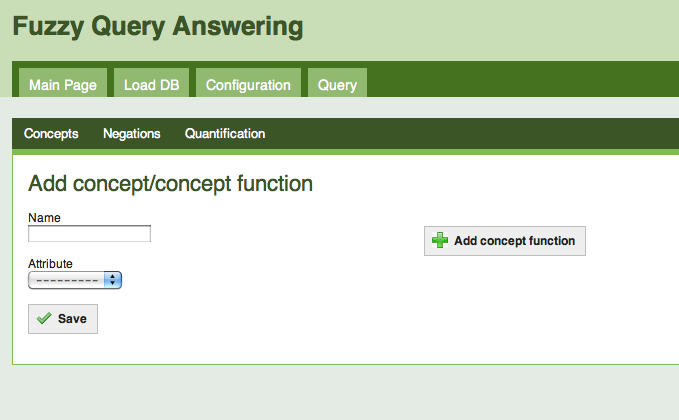
\includegraphics[scale=0.6]{AddingNewConcept.png}
\end{center}
\caption{Interface of adding new concept}
\label{fig:AddNewConceptInterface}
\end{figure}
As shown in figure \ref{fig:AddNewConceptInterface}, users can give the name of fuzzy concepts in ``Name" edit box, and choose an attribute from ``Attribute" selection box. For example, putting ``big" in ``Name" edit box and choosing ``size" from ``Attribute" selection box, in order to create a concept ``big" over attribute ``size". User can continue to add concept functions for this fuzzy concept by clicking ``Add concept function" in the case of adding functions for this fuzzy concept, then save both fuzzy concept and its functions. 
\newpage
\begin{figure}[h]
\begin{center}
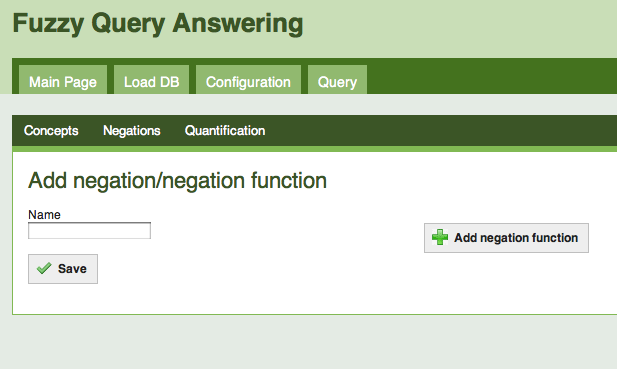
\includegraphics[scale=0.6]{AddingNewNegation.png}
\end{center}
\caption{Interface of adding new negation}
\label{fig:AddNewNegationInterface}
\end{figure}
As shown in figure \ref{fig:AddNewNegationInterface}, adding negation and adding quantification are the same, users only need to type the name of negation or quantification and click button ``Save". Before saving, users can also add functions of negation or quantification by clicking ``Add negation function" or ``Add quantification function".
 \newpage
\begin{figure}[h]
\begin{center}
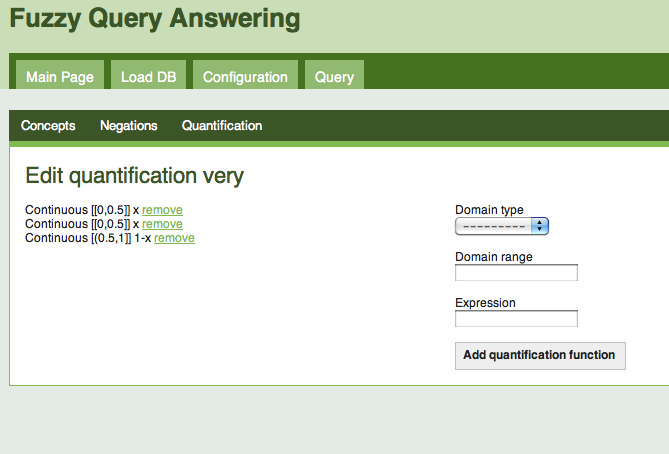
\includegraphics[scale=0.6]{EditingQuantification.png}
\end{center}
\caption{Interface of editing quantification}
\label{fig:EditQuantification}
\end{figure}
For editing functions, it is the same for fuzzy concepts, negations, and quantifications. As shown in figure \ref{fig:EditQuantification}, users can click hyperlink ``edit functions" behind the fuzzy concept, negation, quantification you want to edit. After entering the page of editing functions, users can remove the certain existing functions by clicking the hyperlink ``remove". In order to add more functions, users can choose the function type  from selection box ``Domain type", and type function domain in edit box ``Domain range", then write function expression in edit box ``Expression", the last step is to click button ``Add quantification function" in the case user edits quantification functions. The new function will be added to the list of functions on the left.


